% Résultats fondamentaux
% ======================

\chapter{Résultats fondamentaux}
\label{sec:r_sultats_fondamentaux}

\section{Algorithmes et effectivité}
\label{sub:algorithmes_et_effectivit_}
Qu'est-ce qu'un algorithme?

\begin{mydef}[Algorithme]
	C'est une procédure qui peut être appliquée à n'importe
	quelle donnée et qui a pour effet de produire un résultat. C'est un ensemble fini
	d'instructions qui peuvent être exécutées. Dans cette partie du cours, on ne prend pas la taille des données, des instructions ni de la mémoire disponible en compte, mais on les considère comme finies.
\end{mydef}

\begin{myrem}
	Un algorithme n'est pas une fonction, mais un algorithme calcule une fonction.
	De plus dans le cours on se limite aux fonctions de $\N^n$ dans $\N$. Car on peut,
	montrer que ça revient au même que de considérer de $\N^n$ dans $\N^n$ (
	$\N^n$ est énumérable et donc au plus de même cardinal que $\N$). On va aussi
	utiliser Java comme modèle étant donné que c'est plus facile et qu'on va montrer
	que les modèles complets sont équivalents.
\end{myrem}

% subsection algorithmes_et_effectivit_ (end)

\section{Fonctions calculables, ensembles récursifs et récursivement énumérables}
\label{sub:fonctions_calculables_ensembles_r_crusids_et_r_cursivement_num_rables}

\subsection{Fonction calculable}
\label{ssub:fonction_calculable}

\begin{mydef}[Fonction calculable]
	Une fonction $f$ est calculable s’il existe un algorithme qui, recevant comme donnée
	n'importe quels nombres naturels $x_1,\ldots,x_n$ fournit \textbf{tôt ou tard} comme
	résultat $f(x)$ s’il existe.
\end{mydef}

S'il ne se termine pas c'est que $f(x)=\perp$.

\begin{myrem}
	Il faut faire la distinction entre la non-existence d'un algorithme
	et ne pas être capable de le trouver.
    (Voir exemple TP et cours : y a-t-il une rose verte sur Mars
    ou encore $x$ occurrences de 5 dans $\pi$).
\end{myrem}

\begin{myrem}
	Une fonction peut-être totale calculable ou partielle calculable.
\end{myrem}

% subsubsection fonction_calculable (end)

\subsection{Ensemble récursif et récursivement énumérable}
\label{ssub:ensemble_r_cursif_et_r_cursivement_num_rable}
Soit $A\subseteq \N$

\begin{mydef}[Ensemble récursif]
	Un ensemble $A$ est récursif s'il existe un algorithme qui recevant un $x\in \N$,
	fournit \textbf{tôt ou tard} comme résultat
	\begin{tabular}{l}
		1 si $x\in A$\\
		0 si $x\notin A$\\
	\end{tabular}
	. L'algorithme décide si $x$ est dans $A$ ou non.
\end{mydef}

\begin{mydef}[Ensemble récursivement énumérable]
	Un ensemble $A$ est récursivement énumérable ($\in RE$) s’il existe un algorithme qui recevant
	un $x\in \N$,
    \begin{itemize}
      \item fourni \textbf{tôt ou tard} comme résultat 1 si $x\in A$.
      \item ne se termine pas ou retourne un résultat $\neq1$ si $x \notin A$.
	\end{itemize}
\end{mydef}

\begin{mydef}[Ensemble co-récursivement énumérable]
  Un ensemble $A$ est \emph{co-récursivement énumérable}
  si son complément $\bar{A} = \N \setminus A$ est récursivement énumérable.
\end{mydef}

\begin{myrem}
	Le souci lorsque c'est récursivement énumérable,
	c'est que même si l'algorithme permet de dire si $x$ est dans $A$, si $x$
	n'est pas dans $A$ on ne sait rien dire. En effet, on ne peut pas dire à un moment qu'on
	arrête l'algorithme et que l'élément n'est pas dans $A$.
       	Car il est possible que $x$ soit dans $A$ et que l'algorithme ne
	l'ait pas encore déterminé (l'algorithme retourne tôt ou tard un
	résultat si $x$ est dans $A$!).
\end{myrem}

\paragraph{Définition importante :}
\label{par:d_finition_importante}

\begin{mydef}[Fonction caractéristique]
	Fonction caractéristique de $A$:
	$X_A \colon \N \to {0,1}$, \\
	tel que
    \[ X_A(x) =
      \begin{cases}
        1 & \text{si }x \in A \\
        0 & \text{si }x \notin A
      \end{cases}
    \]
\end{mydef}

\begin{myprop}
	$A$ est un ensemble récursif ssi $X_A$ est une fonction totale	calculable.

    On remarque en effet que $X_A$ décide si $x$ appartient à $A$ ou non.
\end{myprop}

\begin{myprop}
	$A$ est un ensemble récursivement énumérable ssi $A = \dom(f)$ et $f$ est une fonction (totale ou partielle) calculable. En effet, tout ensemble récursif est récursivement énumérable (Propriété 25 ci-dessous).

    \begin{proof}
      Comme $f$ est calculable,
      il existe un programme $P_f$ qui calcule $f$.
      On peut alors construire un programme $Q$ qui avec input $x$,
      appelle $P_f$.
      Si $P_f$ ne se termine pas($P_f(x) = \bot$) alors $Q$ non plus ($Q(x)= \bot$) mais si $P_f$ termine, alors $Q$ renvoie 1.
    \end{proof}
\end{myprop}

\begin{myprop}
	$A$ est un ensemble récursivement énumérable ssi
    \begin{itemize}
      \item $A$ est vide ou
      \item $A = \image(f)$ et $f$ est une fonction totale calculable.
    \end{itemize}

    \begin{proof}
      $f$ est une fonction d'énumération (elle peut répéter plusieurs fois un élément, mais ce n'est pas gênant).
      À l'aide d'un programme $P_f$ qui calcule $f$,
      on appelle $P_f(0), P_f(1), P_f(2), \ldots$
      jusqu'à ce que $P_f(k) = x$ où on retourne $1$.
      Si $x \in \image(f)$, on retournera $1$ tôt ou tard.
      Sinon, on ne terminera jamais, ce qui équivaut à retourner $\bot$.
    \end{proof}
\end{myprop}

% paragraph d_finition_importante (end)

\paragraph{Propriétés importantes}
\label{par:propri_t_s_importantes}
\begin{myprop}
	$A$ récursif $\Rightarrow$ $A$ récursivement énumérable. (Propriété plus
		faible)
\end{myprop}

\begin{myprop}
	$A$ récursif $\Rightarrow$ ($\N \setminus A$) récursif.\\ On peut facilement créer
		un programme qui retourne 1 - le programme qui décide $A$.
\end{myprop}

\begin{myprop}
    Si $A$ est récursivement énumérable et co-récursivement énumérable ($\stcomp{A}$ recursivement énumérable)
    alors $A$ est récursif.
    \begin{proof}
      Il suffit de créer un programme $Q$ qui, pour décider récursivement si $x \in A$, appelle le programme qui décide $A$ et le programme qui décide $\stcomp{A}$ dans deux threads et renvoie 1 si $x \in A$ et 0 si $x in \stcomp{A}$. En effet, si $A$ et $\stcomp{A}$ sont récursivement énumérables, un des deux appels finira tôt ou tard par dire si x appartient à $A$ ou non.
    \end{proof}
\end{myprop}

\begin{myprop}
	$A$ fini $\Rightarrow$ $A$ récursif.
    \begin{proof}
      Si l'ensemble est $a_0, \ldots, a_n$, le programme suivant marche
      \begin{algorithmic}
        \IF{$x = a_0$}
        \STATE print 1
        \ELSIF{$x = a_1$}
        \STATE print 1
        \STATE ...
        \ELSIF{$x = a_n$}
        \STATE print 1
        \ELSE
        \STATE print 0
        \ENDIF
      \end{algorithmic}
    \end{proof}
\end{myprop}
% Une fonction dont le domaine est un ensemble récursif en input est-elle calculable: non

\begin{myprop}
	($\N \setminus A$) fini $\Rightarrow$ $A$ récursif. (Trivial)
\end{myprop}

\begin{myexem}
  Existe-t-il une fonction $f$ qui renvoie 1 s'il existe au moins $x$ occurrences successives de 5 dans $\pi$.

  Oui, c'est soit
  \begin{algorithmic}
    \STATE print 1
  \end{algorithmic}
  s'il y a une infinité de $5$ dans $\pi$,
  soit
  \begin{algorithmic}
    \IF{$x \leq a$}
    \STATE print 1
    \ELSE
    \STATE print 0
    \ENDIF
  \end{algorithmic}
  si il y a exactement $a$ occurrences de $5$ and $\pi$.

  Si on remplace ``au moins'' par ``exactement'', est-ce toujours calculable ?
  Oui, il suffit de remplacer $\leq$ par $=$.
\end{myexem}

\begin{myprop}
  Tout programme qui a un nombre fini d'input différent est calculable (ça ne marche pas s'il est infini car le taille du code du programme doit être fini donc on ne peut pas tout hardcoder).
\end{myprop}

% paragraph propri_t_s_importantes (end)
% subsubsection ensemble_r_cursif_et_r_cursivement_num_rable (end)
% subsection fonctions_calculables_ensembles_r_crusids_et_r_cursivement_num_rables (end)

\section{Thèse de Church-Turing}
\label{sub:th_se_de_church_turing}
Grâce à la définition, on sait montrer qu'une fonction est calculable. Mais comment
montrer qu'une fonction n'est pas calculable? Pour ça on a besoin d'une définition
couvrant la totalité des fonctions calculables.

Une autre question est : "Est-ce que prendre un modèle particulier est restrictif?"

La thèse de Turing répond à ces questions.
\begin{enumerate}
	\item Aucun modèle de la notion de fonction calculable n'est plus puissant que les Machines de Turing.
		Version moderne : Une fonction est calculable s'il existe un programme d'ordinateur qui calcule cette fonction.
	\item Toute fonction calculable est calculable par une machine de Turing.
	\item Toutes les définitions formelles de la calculabilité connues à ce jour sont équivalentes (Théorème, ça a été démontré) (justifie l'utilisation de Java comme modèle).
	\item Toutes les formalisations de la calculabilité établies par la
		suite seront équivalentes aux définitions connues
\end{enumerate}
1, 2 et 4 sont des thèses universellement reconnues comme vraies et la 3 est un théorème.

% subsection th_se_de_church_turing (end)

\section{Programmes et fonctions}
\label{sub:programmes_et_fonctions}
Dans le cours on utilise un langage de programmation, Java, comme modèle.

\begin{mydef}[P]
	Soit P l'ensemble des programmes Java qui reçoit un ou plusieurs entiers comme donnée(s) et qui imprime/retourne un résultat.
\end{mydef}

\begin{myprop}
	P est un ensemble infini dénombrable, car c'est chaîne de caractère d'un alphabet fini. P est récursif, car il existe un programme, le compilateur, qui détermine si un programme est un programme Java ou non.
\end{myprop}

\begin{mydef}[Énumération de P]
	P = $P_0$, $P_1$,... ,$P_k$,... est l'énumération des programmes Java sans répétition. Ce qui implique qu'on peut numéroter les programmes Java.\\
\end{mydef}

\begin{mydef}[$P_k$]
	$P_k$ est le programme numéro $k$ dans $P$
\end{mydef}

\begin{mydef}[$\phi^{(n)}_k$]
	$\phi^{(n)}_k$ : $\N^n \rightarrow \N$ est la fonction calculée par $P_k$
\end{mydef}

\begin{myrem}
  $P_{12} \neq P_{47}$ mais ça ne veut \emph{pas} dire que $\phi_{12} \neq \phi_{47}$. En effet, il existe une infinité de manière de coder une fonction.
\end{myrem}

\begin{myprop}
	Il existe donc une fonction $f : \N\rightarrow P$ telle que :
	\begin{itemize}
		\item $f(k) = P_k$
		\item $f$ calculable
		\item $k$ (numéro d'un programme) et $P_k$ sont deux représentations
			distinctes d'un même objet.
	\end{itemize}
\end{myprop}

% subsection programmes_et_fonctions (end)

\section{Existence de fonctions non calculables}
\label{sub:existence_de_fonction_non_calculables}
Il existe beaucoup de fonctions non calculables, car le nombre de fonctions de $\N$ dans $\N$ est non dénombrable (Exemple~\ref{exem:fNN}).
Or le nombre de programmes Java est dénombrable.
Donc il y a beaucoup de fonctions qui ne sont pas calculables.

On ne va s'intéresser qu'aux fonctions qui sont définies par une table finie ou une table infinie que l'on peut décrire de façon finie (on n'est pas capable d'écrire une définition infinie). Il en existe une infinité dénombrable.

On va maintenant montrer que ce n'est pas parce que la table d'une fonction est définie de manière finie que la fonction est nécessairement calculable (exemple la fonction halt qui détermine si un programme se termine ou non).

% subsection existence_de_fonction_non_calculables (end)

\section{Problème de l'arrêt}
\label{sub:probl_me_de_l_arr_t}

\begin{mydef}[halt]
	halt est la fonction : P x $\N$ $\rightarrow$ $\N$ telle que \\
	\begin{tabular}{rl}
	  halt(n, x) = 1 & si $P_n(x)$ se termine \\
	  halt(n, x) = 0 & sinon \\
	  ce qui équivaut à &\\
	  halt(n, x) = 1 & si $\phi_n(x)\neq \perp$ \\
	  halt(n, x) = 0 & sinon \\
	\end{tabular}
\end{mydef}

\begin{myprop}
	halt est une fonction bien définie, totale et sa table est infinie, mais décrite de manière finie. Or on va montrer que halt n'est pas calculable par diagonalisation (comme pour la démonstration de Cantor).\\
\end{myprop}

\begin{myrem}
	Attention, juste dire qu'on ne sait pas écrire un programme qui calcule halt ne prouve pas qu'on ne sait pas calculer halt. En effet, comme vu dans le chapitre 1, prouver que le programme existe est différent de savoir écrire le programme.
\end{myrem}

\begin{mytheo}[halt]
	halt n'est pas calculable
\end{mytheo}

\paragraph{Démonstration :}
On suppose halt calculable.
\begin{enumerate}
	\item On peut donc construire une table infinie définissant la fonction
		halt : \\
		\begin{tabular}{|c||c|c|c|c|c|c|}
			\hline
			& 0 & 1 & 2 & ... & k & ... \\
			\hline
			$p_0$ & $halt(0,0)$ & $halt(0,1)$ & $halt(0,2)$ & ... & $halt(0,k)$ & ... \\
			$p_1$ & $halt(1,0)$ & $halt(1,1)$ & $halt(1,2)$ & ... & $halt(1,k)$ & ... \\
			$p_2$ & $halt(2,0)$ & $halt(2,1)$ & $halt(2,2)$ & ... & $halt(2,k)$ & ... \\
			: & : &:& : & : & : &:\\
			$p_k$ & $halt(k,0)$ & $halt(k,1)$ & $halt(k,2)$ & ... & $halt(k,k)$ & ... \\
			: & : &:& : & : & : &:\\
			\hline
		\end{tabular}
	\item Sélection de la diagonale
		\[ diag :halt(0,0),halt(1,1),...,halt(k,k),... \]
		\[diag(n) = halt(n,n)\]
	\item Modification de cet élément diag pour obtenir
		$diag'(n) =$
		\begin{tabular}{c}
			1 si halt(n,n) = 0\\
			$\perp$ si halt(n,n) = 1\\
		\end{tabular}\\
		$diag'$ est calculable, car halt est calculable (il y a moyen
		d'écrire un programme qui calcul $diag'$ en utilisant $diag$)
	\item Contradiction :\\
	       	Donc il existe un programme $P_d$ qui calcule
		$diag'$:
		$diag'(d) =$
		\begin{tabular}{c}
			1 si halt(d,d) = 0\\
			$\perp$ si halt(d,d) = 1\\
		\end{tabular}
		Mais,
		\begin{itemize}
			\item Si $diag'(d)= 1$ $\\
			\Rightarrow \  halt(d,d) = 0 \\
			\Rightarrow \ P_d(d)$ ne se termine donc pas $ \\
			\Rightarrow diag'(d)$ ne se termine pas $ \\
			\Rightarrow diag'(d) = \perp$ or on a supposé que $diag'(d) = 1$ $ \\
			\Rightarrow $
			Contradiction.

			\item Si $diag'(d)= \perp$ $\\
			\Rightarrow \  halt(d,d) = 1 \\
			\Rightarrow \ P_d(d)$ se termine $ \\
			\Rightarrow diag'(d)$ termine $ \\
			\Rightarrow diag'(d) = 1$ or on a supposé que $diag'(d) = \perp$ $ \\
			\Rightarrow $
			Contradiction.
		\end{itemize}
	\item Conclusion : $diag'$ n'est pas calculable $ \Rightarrow $ $diag$
	n'est pas calculable $ \Rightarrow $ halt n'est pas calculable.

\end{enumerate}

\paragraph{Conclusion} Il n'existe pas d'algorithme qui détermine si n'importe quel programme $P_n$ se termine ou non. Mais dans certains formalismes qui ne sont pas des modèles complets la fonction halt de ce formalisme est calculable.
Par exemple un langage qui ne permet de calculer
que des fonctions totales (exemple java sans aucune boucle), halt est calculable (halt retourne toujours 1). \\

De plus, il faut faire attention, car ce n'est pas parce que halt n'est pas calculable que pour un programme donné k, $halt(k,x)$ est non calculable. Par exemple $halt(32,123)$ est une fonction constante donc calculable (ce n'est pas pour autant qu'on est capable d'écrire l'algorithme), $halt(32,x)$ peut-être calculable, mais ça dépend du programme 32, par exemple si celui-ci est constant.

\begin{myrem}
	Cette partie du cours est très importante, car on a trouvé un ``trou dans le mur des fonctions calculables'' et on va étendre le trou (métaphore
	de Mr Deville). C'est-à-dire que maintenant on va utiliser halt pour montrer que d'autres fonctions sont calculables/non calculables. Par exemple	par réduction par rapport à halt: si on montre qu'une fonction équivalente à halt est calculable, alors halt est calculable.
\end{myrem}

Il existe donc au moins un ensemble non récursif
K.

\begin{mydef}[K]
	K =
	\begin{tabular}{l}
		\{n|(n,n)$\in$ HALT\}\\
		\{n| halt(n,n)=1\}\\
		\{n| $P_n(n)$ se termine\}
	\end{tabular}
	$K$ est donc l'ensemble des programmes $P_n$ qui se terminent en recevant comme entrée leur numéro de programme.
\end{mydef}

\begin{mydef}[HALT]
	HALT est l'ensemble des programmes k et des valeurs x tel que le programme k se termine avec l'entrée x.
	\[ HALT = \{(n,x)|P_n(x)\text{se termine}\}\]
\end{mydef}

\begin{myprop}
	K et HALT ne sont pas récursifs
\end{myprop}

\begin{myprop}
	K et HALT sont récursivement énumérables (car il suffit de lancer le programme et s’il retourne quelque chose il se termine sinon on ne peut rien dire).
\end{myprop}

\begin{myprop}
	$\stcomp{HALT}$ n'est pas récursivement énumérable sinon HALT serait récursif.  En effet, on ne peut pas coder un programme qui dirait si un autre programme k, appelé avec la valeur x, ne terminera jamais.
\end{myprop}

\begin{myprop}
	$\stcomp{K}$ n'est pas récursivement énumérable
\end{myprop}

\begin{figure}[h]
  \centering
  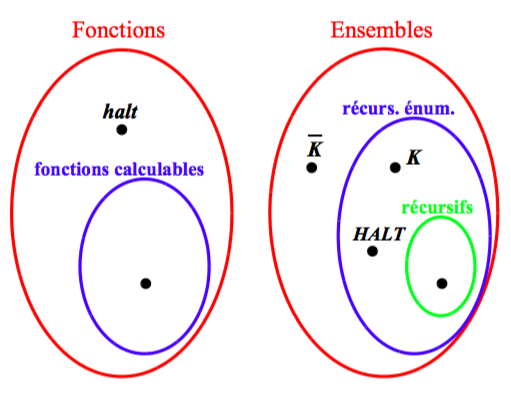
\includegraphics[width=0.57\textwidth]{Images/Structures_de_fonctions_et_ensembles}
  \caption{ Structures de fonctions et ensembles}
  \label{rb}
\end{figure}

%\begin{mydef}[Un ensemble co-récursivement énumérable] est un ensemble dont le complément est récursivement énumérable. Par exemple $stcomp{HALT}$. On peut en déduire que si un ensemble est récursivement énumérable et co-récursivement 	énumérable alors il est récursif.
%\end{mydef} % déjà défini plus haut.

% subsection probl_me_de_l_arr_t (end)

\section{Insuffisance des fonctions totales}
\label{sub:insuffisance_des_fonctions_totales}
Dans un modèle de calcul (langage de programmation) dans lequel tous les programmes se terminent, la fonction halt est triviallement calculable (fonction constante 1).  Etant donné que les problèmes pratiques que l'on doit résoudre sone des fonctions totales, on peut se demander.  Mais on va montrer qu'un tel modèle est restrictif; il ne permet pas de calculer toutes les fonctions totales calculables.

\begin{myexem}
Un exemple de modèle de calcul ne permettant que le calcul de fonctions totales est par exemple BLOOP (défini plus loin) ou encore MiniJava, c'est-à-dire Java sans récursivité ni boucle while et où les boucles for ne peuvent modifier le compteur de boucle. 
\end{myexem}

Posons Q un langage (\textbf{non trivial}) dont tous les programmes se terminent (ils ne calculent que des fonctions totales) et pour
lequel il existe un interpréteur calculable, interpret(n,x)${} =\phi'_n$, où 
$\phi'_n$ est la fonction calculée par le programme $Q_n$.  L'interpréteur est une fonction totale car il donne toujours une réponse vu que tous les programmes se terminent. Par langage de programmation non trivial, on entend un langage où les opérations de base telles que l'addition peuvent être réalisées.

\begin{mytheo}[Hoare-Allison]
	\label{Hoare_Allison}
Soit Q un langage de programmation (\textbf{non trivial}) dans lequel tous les programmes se terminent.	Alors l'interpreteur de Q, la fonction interpret(n,x), n'est pas calculable dans Q.
\end{mytheo}

\paragraph{Démonstration :}
On suppose interpret calculable dans Q.
\begin{enumerate}
	\item On construit une table infinie, où chaque ligne correspond à un programme $Q_k$ de Q.   : \\
		\begin{tabular}{|c||c|c|c|c|c|c|}
			\hline
			& 0 & 1 & 2 & ... & k & ... \\
			\hline
			$Q_0$ & $interpret(0,0)$ & $interpret(0,1)$ & $interpret(0,2)$ & ... & $interpret(0,k)$ & ... \\
			$Q_1$ & $interpret(1,0)$ & $interpret(1,1)$ & $interpret(1,2)$ & ... & $interpret(1,k)$ & ... \\
			$Q_2$ & $interpret(2,0)$ & $interpret(2,1)$ & $interpret(2,2)$ & ... & $interpret(2,k)$ & ... \\
			: & : &:& : & : & : &:\\
			$Q_k$ & $interpret(k,0)$ & $interpret(k,1)$ & $interpret(k,2)$ & ... & $interpret(k,k)$ & ... \\
			: & : &:& : & : & : &:\\
			\hline
		\end{tabular}
	\item Sélection de la diagonale
		\[diag(n) = interpret(n,n)\]
	\item Modification de cet élément diag pour obtenir
		$diag'(n) = interpret(n,n)+1$
		$diag'$ est calculable dans Q, car interpret est calculable dans Q (il y a moyen
		d'écrire un programme qui calcule $diag'$ en utilisant $diag$)
	\item Contradiction :\\
	       	Comme $diag'$ est calculable dans Q, il existe un programme $Q_d$ qui calcule $diag'$.  
		Mais quelle est la valeur de $diag'(d)$ ?
		Par définition de $diag'$, on a $diag'(d) = interpret(d,d)+1$. \\
		Mais, comme $Q_d$ calcule $diag'$, par définition $diag'(d) = Q_d(d) = \phi_d(d) = interpret(d,d)$.
		En effet, calculer $\phi_d(d)$ revient à interpréter le programme
		d avec la donnée d. \\
		On obtient donc $interpret(d,d)+1 = interpret(d,d)$, ce qui est impossible car $interpret(d,d)$ est un entier. 
	\item Conclusion : $diag'$ n'est pas calculable dans $Q$, donc $diag$
	n'est pas calculable dans Q, et donc interpret n'est pas calculable dans $Q$.
dans Q.
\end{enumerate}

\begin{myrem}
	Si les programmes de Q ne calculaient pas que des fonctions totales, alors ça n'aurait pas posé de problèmes, car si $interpret(d,d)=\bot$, $interpret(d,d)+1=\bot$ et il n'y a plusa de contradiction.  Un programme qui ne se termine pas + quelque chose, reste un programme qui ne se termine pas.
\end{myrem}



\subsection{Implication du théorème \ref{Hoare_Allison}, Hoare Allison }

\begin{myprop}
	Si un langage (\textbf{non trivial}) ne permet que le calcul de fonctions totales, alors :
	\begin{itemize}
		\item l'interpréteur de ce langage n'est pas calculable dans ce langage.
		\item il existe des fonctions totales non programmables dans ce langage.
		\item ce langage est \bf{restrictif}.
	\end{itemize}
\end{myprop}

\begin{myprop}
	Si on peut programmer l'interpréteur d'un langage L dans L alors il est
	impossible de programmer la fonction halt dans L car celle-ci n'est pas calculable.
\end{myprop}

\begin{myprop}
	Dans un langage de programmation, il est donc impossible que
	l'interpréteur et la fonction halt puissent être programmés dans ce langage.
\end{myprop}

\begin{myprop}
	Si on veut pouvoir programmer toutes les fonctions totales dans un langage, le langage doit permettre la programmation de fonctions non totales.
\end{myprop}

\begin{myprop}
	L'ensemble \{n| $\phi_n$ est totale\} n'est pas récursif.
    (sinon on saurait créer un langage qui calcule toutes les fonctions totales et uniquement les fonctions totales).
\end{myprop}

\begin{mytheo}[fonction universelle]
  \label{theo:fununiv}
	La fonction universelle (c'est-à-dire l'interpréteur) est $\theta(n,x)$ tel que :
	\[ \theta(n,x) = \phi_n(x) \]
    est calculable, c'est à dire qu'il existe $z$ tel que $P_z$ calcule l'interpréteur universel,
    c'est à dire $\phi_z = \theta$.
\end{mytheo}

% subsection insuffisance_des_fonctions_totales (end)

\section{Extension de fonctions partielles}
\label{sub:extension_de_fonctions_partielles}

\begin{mytheo}
	Il existe une fonction partielle calculable g telle qu'aucune fonction totale calculable n'est une extension de g.
  \begin{proof}
    C'est le cas de $\diag'$ avec le tableau $\interpret(i,j)$ (le même que pour la preuve avec $Q$). S'il existe une extension calculable $f = \phi_s$ de $\diag'$,
    alors si $\interpret(s,s) = \bot$, $\phi_s(s) = \diag'(s) \neq \bot = \interpret(s,s)$, c'est une contradiction
    et si $\interpret(s,s) \neq \bot$, $\phi_s(s) = \diag'(s) = \diag(s)+1 = \interpret(s,s)+1 \neq \interpret(s,s)$,
    c'est une contradiction.

    On en conclut que la fonction universelle n'est pas calculable, ce qui contredit le théorème~\ref{theo:fununiv}.
  \end{proof}
\end{mytheo}

\begin{myrem}
	Ca implique que si on a une fonction partielle g, il n'est pas
	toujours possible de créer une fonction totale f qui étend g
	tel que en dehors du domaine de g, f retourne un code d'erreur.  En effet, si cette fonction f existait, halt serait calculable.
\end{myrem}

% subsection extension_de_fonctions_partielles (end)

\section{Théorème de Rice}
\label{sub:th_or_me_de_rice}

Soit A $\subseteq$ $\N$

\begin{mytheo}[Rice]
	Si $A$ récursif et $A\neq \emptyset$ et $A \neq \N$ \\
	Alors $\exists i \in A$ et $\exists j \in \N \setminus A$ tels que $\phi _i = \phi _j$
\end{mytheo}

On utilise le plus souvent le théorème de Rice en ayant recourt à sa contraposée:

\begin{mytheo}[Rice (contraposée)]
	Si $\forall  i \in A$ et $\forall j \in \stcomp{A}$ on a $\phi_i \neq \phi_j$ \\
	Alors $A$ non-récursif ou $A = \emptyset$ ou $A = \N$
\end{mytheo}

Dans de nombreux cas, on peut garantir $A \neq \emptyset$ et $A \neq \N$, ce qui permet de se servir de la contraposée pour démontrer qu'un ensemble est non-récursif sans utiliser la preuve par diagonalisation ou par réduction.

\begin{proof}
On a $\forall i \in A$ et $\forall j \in \stcomp{A}$ tel que $\phi_i \neq
\phi_j$\\
Supposons $A$ récursif, $A \neq \emptyset$ et $A\neq \N$\\
On va montrer que HALT est récursif, car on peut construire un programme qui
décide HALT, alors qu'on sait que HALT n'est pas récursif.

\begin{enumerate}
	\item Construisons le programme $P_k$
\begin{lstlisting}
while true do;
\end{lstlisting}
	$\forall x \ \phi_k(x) = \perp$
	\item $\stcomp{A}\neq \emptyset$ car $A \neq \N$,
	supposons $k\in \stcomp{A}$ (hypothèse sans importance, car montrer que
	$A$ ou $\stcomp{A}$ est non récursif revient au même, car $A$ non
	récursif $ \Leftrightarrow $ $\stcomp{A}$ non récursif)
	\item $A\neq \emptyset$ par hypothèse, supposons $m\in A$
	\item $\phi_i \neq \phi_j$ et ce $\forall i \in A, \forall j \in \stcomp{A}$ par hypothèse donc
		$\phi_m \neq \phi_k$
	\item Construisons un programme $P(z)$ qui calcule la fonction $g(z)$,
		$P(z) \equiv $
\begin{lstlisting}
P_n(x);
P_m(z);
\end{lstlisting}
	\begin{myrem}
		On sait que si un programme calcule une fonction $
		f(x)=\perp \ \forall x$ alors ce programme doit être dans $\stcomp{A}$ car
		$f(x) =\phi_k(x)$.

		Or
		\begin{itemize}
			\item soit notre programme $P(z)$ ne se termine pas $\forall z$, car $P_n(x)$ ne se termine pas et donc $g(z) = 		\phi_k(z)$.
		\item soit notre programme $P(z)$ calcule $\phi_m(z)$ or on
			sait que $m\in A$.
		\end{itemize}
        Donc en résumé si $P_n(x)$ ne se termine pas $P(z)$ sera dans
        $\stcomp{A}$ sinon $P(z)$ sera dans $A$.
	\end{myrem}
	Un programme qui décide HALT $halt(n,x) \equiv $
\begin{lstlisting}
construire P(z);
d <- numero de P(z);
if d in A then print(1);
else print(0);
\end{lstlisting}
	\item Contradiction, car HALT n'est pas récursif.
	\item Conclusion: $A$ n'est pas récursif.
\end{enumerate}
\end{proof}

\paragraph{} On est intéressé par l'analyse des propriétés d'un programme. Est-ce que ces propriétés peuvent être déterminées par un
algorithme? On va utiliser le théorème de Rice pour différencier les propriétés
qu'il est possible de déterminer par un algorithme de celles pour lesquelles ce
n'est pas possible.

\paragraph{}Pour ça, considérons $A$ comme étant l'ensemble des programmes qui
respectent une propriété. Par exemple $A_1 = \{i| \phi_i \text{ est total}\}$ ou
$A_2=\{i|\phi_i = f\}$,... (il y a plein d'exemples dans le cours).

\paragraph{Analyse}
\begin{itemize}
	\item Si la propriété est vérifiée par certains programmes, mais pas tous,
		et qu'elle est décidable, alors il existe deux programmes calculant la
		même fonction, mais l'un vérifie la propriété, et l'autre pas.

	\item Si la propriété est vérifiée par un programme, mais pas tous,
		alors cette propriété ne peut-être décidée pas un algorithme.

	\item S'il existe un algorithme permettant de déterminer si un
		programme quelconque calcule une fonction ayant cette propriété,
		alors toutes les fonctions calculables ont cette propriété ou
		aucune fonction calculable n'a cette propriété.

	\item Aucune question relative aux programmes, vu sous l'angle de la
		fonction qu'ils calculent, ne peut être décidée par
		l'application d'un algorithme.

	\item Les propriétés intéressantes d'un programme concernant la
		fonction qu'il calcule, non pas sa forme,
		sont non calculables.
\end{itemize}


% subsection th_or_me_de_rice (end)

\section{Théorème de la paramétrisation}
\label{sub:th_or_me_de_la_param_trisation}

\subsection{Transformation de programmes}
\label{ssub:transformation_de_programmes}
\begin{mydef}[Transformateur de programme]
	On peut voir une fonction f: $\N \rightarrow \N$ comme une fonction qui prend
	le numéro d'un programme et qui retourne le numéro d'un autre programme f: $P
	\rightarrow P$. Donc on peut voir $P_k$, le programme qui calcule f comme un
	transformateur de programme. En effet, $P_k$ prend un programme en entrée et
	retourne un programme qui peut être différent.
\end{mydef}

\begin{mytheo}[S-m-n]
	\label{S-m-n}Pour tout $m,n \geq 0$, \\
	il existe une fonction totale calculable $S^m_n : \N^{m+1} \rightarrow
	\N$ \\
	telle que pour tout $k$ ($\phi_k$ est calculable),
	$$ \phi^{(n+m)}_k(x_1,...,x_n,x_{n+1},...,x_{n+m}) =
	\phi^{(n)}_{S^m_n(k,x_{n+1}, ...,x_{n+m})} (x_1,...,x_n)$$
\end{mytheo}

\begin{proof}
	Pour prouver que $S^m_n$ est totale calculable, on va montrer comment construire un programme qui
	calcule  $S^m_n(k,x_{n+1}, ...,x_{n+m})$.\\
	Tout d'abord, comme $\phi_k$ est calculable, il existe un programme
	$P_k(x_1,x_2,...,x_{n+m})$.\\
	On peut donc construire un programme $Q(x_1,...,x_n)$ qui calcule
	$P_k(x_1,x_2,...,x_{n+m})$.\\
	$x_1,...,x_n$ restent des arguments du programme,
	tandis que $x_{n+1},...,x_{n+m}$ deviennent des valeurs fixées.\\
	Notre programme qui calcule $S^m_n(k,x_{n+1}, ...,x_{n+m})$ n'a plus
	qu'à retourner le numéro du programme $Q$.\\
       	En résumé, $S^m_n(k,x_{n+1},
	...,x_{n+m}) \equiv$
	\begin{lstlisting}
construire Q(x1,x2,...,xn) = P_k(x1,x2,...xn,...,xn+m);
d <- numero du programme Q;
print(d);
	\end{lstlisting}
\end{proof}

\begin{mytheo}[S]
	C'est la propriété S-m-n affaiblie.
	\[ \forall \ k \ \exists \ S \ \text{(totale calculable)} : \phi_k(x,y)=\phi_{S(y)}(x)\]
	% Lena : j'ai plutôt ceci (c'est équivalent)
	% $$ \forall \text{ programme } P, \exists S \text{ totale calculable }:
	% P(x,y) \equiv \left[S(y) \right](x) $$
\end{mytheo}

\paragraph{Démonstration}
	Par le théorème \ref{S-m-n} (S-m-n),
	\[ \exists \ S \text{ (totale calculable) } \forall \ k : \phi_k(x,y)=\phi_{S(k,y)}(x)\]
	\[ \forall \ k \ \exists \ S \ \text{ (totale calculable) } : \phi_k(x,y)=\phi_{S(k,y)}(x)\]
	\[ \Rightarrow \forall \ k \ \exists \ S : \phi_k(x,y) =\phi_{S(k,y)}(x) \]
	\begin{align}
		\Rightarrow S(k,y) &= \phi_{S}(k,y) \text{ (S est totale calculable)}\\
		&= \phi_{S'(S,k)}(y) \text{ (S-m-n)}\\
		&= \phi_{k'}(y) \text{ (renomage de } S'(S,k) \text{ en } k' \text{)}\\
		&= S''(y)
	\end{align}
	\[ \Rightarrow \forall \ k \ \exists \ S'' \ \text{(totale calculable)} :
       	\phi_k(x,y)=\phi_{S''(y)}(x)\]

\begin{myrem}
	On peut voir le théorème \ref{S-m-n}, S-m-n, comme : \\
	Étant donné $m,n \geq 0$\\
	il existe un transformateur de programme, $S^m_n$, qui recevant comme
	données : un programme $P_k$ à $n+m$ arguments et $m$ valeurs $v_1,...,v_m$
	fournit comme résultat: un programme $P$ à $n$ arguments tel que
	$P(x_1,...,x_n)$ calcule la même fonction que
	$P_k(x_1,...,x_n,,v_1,...,v_m)$ (Ce programme effectue une projection)
\end{myrem}

\begin{myrem}
	On peut donc voir la transformation de programmes $S^m_n$ comme un
	programme qui particularise un autre programme à $m+n$ argument en rendant
	constant les m derniers paramètres.
\end{myrem}

\section{Théorème du point fixe}
\label{sub:th_or_me_du_point_fixe}
\begin{mytheo}[Point fixe]
	\label{point-fixe}
    Soient $n \geq 0$ et $f$ : fonction totale
	calculable, il existe $k$ tel que $\phi^{(n)}_k = \phi^{(n)}_{f(k)}$
\end{mytheo}

%TODO Démonstration avec les lapins (les 3 lapins qui permettent
%de commencer la démonstration ne sont pas super intuitifs)
\begin{myrem}
	Le théorème \ref{point-fixe} n'est pas très intuitif. Mais on peut le
	voir comme : quel que soit un transformateur de programme T qui calcule f (n'importe quelle fonction totale calculable peut être vu comme un transformateur	de programme),
	il existe deux programmes $P_k$ et $P_j$ tels que
	\begin{itemize}
		\item $P_j$ est la transformation de $P_k$ via T,
		\item $P_k$ et $P_j$ calcule la \textbf{même} fonction.
	\end{itemize}
\end{myrem}

\begin{proof}
Pour commencer, on va poser 3 ``lapins'' :
\begin{enumerate}
	%\item $h(u,v) =$
	%	\begin{tabular}{c}
	%		$\phi_{\phi_{u(u)}}(v)$ si $\phi(u)\neq \perp$\\
	%		$\perp$ sinon
	%	\end{tabular}\\

	\item
	$ h(u,v) = \left\{
	\begin{array}{l l}
		\phi_{\phi_{u}(u)}(v) & \quad \text{si $\phi_u(u)\neq \bot$}\\
    	\bot & \quad \text{sinon}
	\end{array} \right.$

		$h$ est calculable
		\begin{myrem}
			on peut créer un programme qui calcule $h$
            \begin{algorithmic}
              \STATE Input: $u,v$
              \STATE $a = P_z(u,u)$
              \STATE $P_z(a,v)$
            \end{algorithmic}
            où $\phi_z = \theta$ est la fonction universelle.
		\end{myrem}

	\item $h(u,v)=\phi_{S(u)}(v)$\\
	 $S$ est totale calculable, on a donc la propriété S (propriété S-m-n affaiblie).

	\item $g(u)=f(S(u))$\\
	 $g$ est totale calculable car $S$ et $f$ le sont ($f$
		est la fonction donnée dans le théorème).
		\[ \exists k' \cdot \phi_{k'}(u) =g(u)=f(S(u)) \]
\end{enumerate}
On a que $k'$ est une constante et par le lapin 2 :
\[h(k',v) = \phi_{S(k')}(v)\]
Par le lapin 1 et, car $g=\phi_{k'}$ est une fonction totale calculable, on a :
\[h(k',v) = \phi_{\phi_{k'}(k')}(v)\]
Par le lapin 3 on a que $\phi_{k'}(u) = g(u)=f(S(u))$ donc :
\[h(k',v) = \phi_{f(S(k'))}(v)\]
C'est à dire :
\[ \phi_{S(k')}(v) =\phi_{f(S(k'))}(v) \]
Si on pose que $S(k')=k$ on a bien
\[ \phi_{k}(v) = \phi_{f(k)}(v) \]
Ce qui conclut notre démonstration.
		\begin{myrem}
          Le programme créé par $S(k')$ est le suivant
          \begin{algorithmic}
            \STATE Input: $v$
            \STATE $a = P_z(k',k')$
            \STATE $P_z(a,v)$
          \end{algorithmic}
          On remarque que comme $S$ et $f$ sont totales,
          $g$ l'est aussi donc $P_z(k',k')$ se terminera toujours.

          Que se passe t'il quand on exécute $S(k')$?
          Comme on l'a vu, la première ligne se termine et on obtient
          $a = f(S(k'))$,
          ensuite on exécute le programme $P_z(a,v) = P_a(f(S(k')),v)$
          et output ce qu'il output.
          Exécuter $S(k')$ revient donc à exécuter $f(S(k'))$!
          On a donc forcément
          \[ \phi_{S(k')} = \phi_{f(S(k'))}. \]
          Le programme $S(k')$ est donc un point fixe de $f$.
		\end{myrem}
\end{proof}

\begin{myrem}[Démonstration du théorème de Rice grâce au point fixe]
  À l'aide du point fixe, on peut démontrer une version plus forte du théorème de Rice:

  Si $A$ est récursif et $A \neq \emptyset \neq \bar{A}$, alors
  il existe $n \in A$ et $m \in \bar{A}$,
  \begin{itemize}
    \item soit $\exists k \in      A $ tel que $\phi_m = \phi_k$
    \item soit $\exists k \in \bar{A}$ tel que $\phi_n = \phi_k$.
  \end{itemize}
  \begin{proof}
    Soit un ensemble $A$ récursif tel que $A \neq \emptyset$ et $\bar{A} \neq \emptyset$.
    Soit $n \in A$ et $m \in \bar{A}$.
    Soit la fonction
    \[
      f(x) =
      \begin{cases}
        m & \text{si }x \in A,\\
        n & \text{si }x \in \bar{A}.
      \end{cases}
    \]
    On remarque que comme $A$ est récursif,
    $f$ est total calculable.
    Dès lors, par le théorème du point fixe, il existe $k$ tel que
    \[ \phi_{f(k)} = \phi_k \]
    \begin{itemize}
      \item Si $k \in A$, ça donne
        \[ \phi_m = \phi_k \]
        or $m \in \bar{A}$.
      \item Si $k \in \bar{A}$, ça donne
        \[ \phi_n = \phi_k \]
        or $n \in A$.
    \end{itemize}
  \end{proof}
\end{myrem}

\begin{myrem}[Démonstration de $K$ grâce au point fixe]
	On peut démontrer que $K$ n'est pas récursif.

    \begin{proof}
	Posons 3 fonctions :
	\begin{itemize}
		\item $\phi_1(x) = \bot \quad \forall \ x$
		\item $\phi_0(x) = x \quad \forall  \ x$
		%\item $f(x) = $
		%	\begin{tabular}{l}
		%		i si $x\in K$\\
		%		j si $x\notin K$\\
		%	\end{tabular}
		\item $ f(x) = \left\{
		\begin{array}{l l}
			1 & \quad \text{si $x\in$ K}\\
    		0 & \quad \text{si $x\notin$ K}
		\end{array} \right.$
	\end{itemize}
    On remarque que par construction pour tout $k$, $\phi_{f(k)} \neq \phi_k$.
    \begin{itemize}
      \item Si $k \in K$, $\phi_k(k) \neq \bot$, $f(k) = 1$ et
        $\phi_{f(k)}(k) = \phi_1(k) = \bot \neq \phi_k(k)$ donc $\phi_{f(k)} \neq \phi_k$.
      \item Si $k \notin K$, $\phi_k(k) = \bot$, $f(k) = 0$ et
        $\phi_{f(k)}(k) = \phi_0(k) \neq \bot = \phi_k(k)$ donc $\phi_{f(k)} \neq \phi_k$.
    \end{itemize}
    Si $K$ est récursif, alors $f$ est total calculable.
	Par le théorème du point fixe, il existe $k$ tel que $\phi_k = \phi_{f(k)}$.
    Ce qui est contradictoire.

    $K$ n'est donc pas récursif.
  \end{proof}
\end{myrem}

\section{Autres problèmes non calculables}
\label{sub:autres_probl_mes_non_calculable}

\begin{mydef}[Problème de correspondance de Post] Soit deux listes U et V
	de mots non vides sur un alphabet $\Sigma$ :
	\begin{itemize}
		\item U = ${u_1,u_2,...,u_k}$
		\item V = ${v_1,v_2,...,v_k}$
	\end{itemize}
	Le problème consiste à décider s’il existe une suite d'entiers
	$i_1,i_2,..,i_n$ telle que les mots $u_{i1},u_{i_2},...,u_{in}$ et
	$v_{i1},v_{i_2},...,v_{in}$ soient \textbf{identiques}. \\
	Pour démontrer l'indécidabilité de ce problème, Post à introduit un
	nouveau modèle, la machine de Post qui ressemble à une machine de Turing.
\end{mydef}

% en français, on écrit ``diophantiennes'', en anglais ``diophantines''
\begin{mydef}[Problème des équations diophantiennes]
  Décider si une équation
  polynomiale de degré supérieur ou égal à 4 possède une solution entière.
\end{mydef}
C'est le 10\ieme{} problème de Hilbert, résolu en 1970 par Matiyasevich;
voir \cite{davis1973hilbert} pour un description de la solution et des remarques historiques.
Ce résultat implique, en particulier, qu'il n'existe pas d'algorithme pour résoudre
la programmation quadratique entière; voir \cite{jeroslow1973there}.
Un bon aperçu des question de non décidabilité pour les équation polynomiale est \cite{koenigsmann2014undecidability}.

Il n'existe pas d'algorithme résolvant ces problèmes. Il existe beaucoup
d'autres problèmes non calculables. Il y a d'autres exemples sur les grammaires dans le cours.
% subsection autres_probl_mes_non_calculable (end)

\section{Nombres calculables}
\label{sub:nombres_calculables}

\begin{mydef}[Nombre réel]
	Un nombre réel est défini comme la limite d'une suite (convergente) de
	nombres rationnels: $\lim_{n \rightarrow +\infty} |x-s(n)| = 0 $ ou s’est
	une fonction totale
\end{mydef}

\begin{mydef}[Nombre réel calculable]
	Un nombre réel x est calculable s’il existe une fonction totale
	calculable $s$ tel que $\lim_{n \rightarrow +\infty} |x-s(n)| \leq 2^{-n}$
\end{mydef}

\begin{myrem}
	Donc un nombre est calculable s'il existe un programme qui peut
	l'approximer aussi près que l'on veut. Par exemple $\pi$ et $e$ sont
	calculable
\end{myrem}

\begin{myprop}
	L'ensemble des nombres réels calculables est énumérable, car on peut énumérer les
	fonctions totales calculables.
\end{myprop}

\begin{myprop}
	Il existe des nombres réels non calculables.
\end{myprop}

\begin{myprop}
	Il existe des nombres réels non calculables qui peuvent être définis de
	manière finie.
\end{myprop}

% subsection nombres_calculables (end)

\section{Conclusion}

Le théorème S-m-n permet de démontrer le théorème du point fixe.
Le théorème du point fixe est un résultat central de la calculabilité. Il
implique le théorème de Rice, la non-récursivité de K et la non-calculabilité
de la fonction halt.

% subsection conclusion (end)
% section r_sultats_fondamentaux (end)

